\begin{figure}[tbp]
\centering
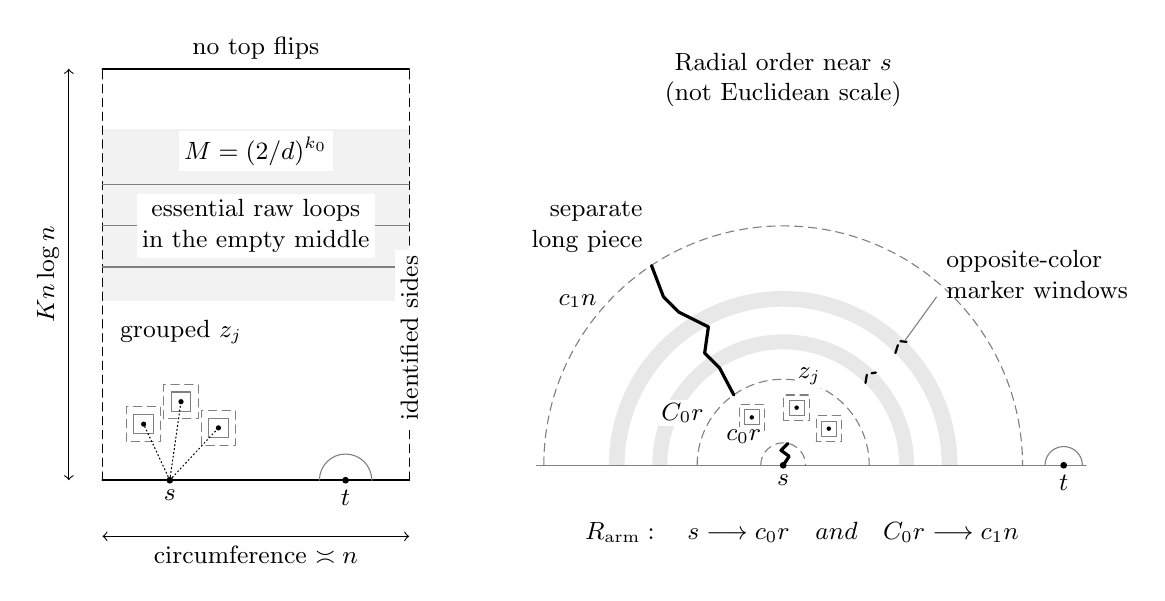
\begin{tikzpicture}[x=.95cm,y=.95cm,font=\small,line cap=round,line join=round]
  \path[fill=gray!10] (0,2.4) rectangle (4.1,4.7);
  \draw[thick] (0,0) -- (4.1,0);
  \draw[thick] (0,5.5) -- (4.1,5.5);
  \draw[densely dashed] (0,0) -- (0,5.5);
  \draw[densely dashed] (4.1,0) -- (4.1,5.5);
  \foreach \y in {2.85,3.4,3.95} {\draw[gray] (0,\y) -- (4.1,\y);}
  \node[fill=white,inner sep=2pt] at (2.05,4.4) {$M=(2/d)^{k_0}$};
  \node[align=center,fill=white,inner sep=2pt] at (2.05,3.4)
    {essential raw loops\\in the empty middle};
  \node[above] at (2.05,5.5) {no top flips};
  \draw[<->] (-.45,0) -- (-.45,5.5);
  \node[rotate=90,above] at (-.45,2.75) {$Kn\log n$};
  \draw[<->] (0,-.75) -- (4.1,-.75);
  \node[below] at (2.05,-.75) {circumference $\asymp n$};
  \fill (.9,0) circle (.045);
  \fill (3.25,0) circle (.045);
  \node[below] at (.9,0) {$s$};
  \node[below] at (3.25,0) {$t$};
  \draw[gray] (2.9,0) arc (180:0:.35);
  \foreach \x/\y in {.55/.75,1.05/1.05,1.55/.7} {
    \draw[gray,densely dashed] (\x-.23,\y-.23) rectangle (\x+.23,\y+.23);
    \draw[gray] (\x-.13,\y-.13) rectangle (\x+.13,\y+.13);
    \fill (\x,\y) circle (.035);
    \draw[densely dotted] (.9,0) -- (\x,\y);
  }
  \node[above] at (1.05,1.7) {grouped $z_j$};
  \node[rotate=90,fill=white,inner sep=2pt] at (4.1,1.9) {identified sides};
  \node[align=center] at (9.1,5.35) {Radial order near $s$\\(not Euclidean scale)};
  \begin{scope}[shift={(9.1,.2)}]
    \foreach \inner/\outer in {1.55/1.75,2.12/2.33} {
      \path[fill=gray!18] (-\outer,0) arc (180:0:\outer)
        -- (\inner,0) arc (0:180:\inner) -- cycle;
    }
    \draw[gray] (-3.3,0) -- (4.05,0);
    \foreach \radius in {.3,1.15,3.2} {
      \draw[gray,densely dashed] (-\radius,0) arc (180:0:\radius);
    }
    \foreach \x/\y in {-.42/.64,.18/.77,.61/.49} {
      \draw[gray,densely dashed] (\x-.17,\y-.17) rectangle (\x+.17,\y+.17);
      \draw[gray] (\x-.1,\y-.1) rectangle (\x+.1,\y+.1);
      \fill (\x,\y) circle (.03);
    }
    \fill (0,0) circle (.045);
    \node[below] at (0,0) {$s$};
    \draw[line width=1.15pt] (0,0) -- (.08,.12) -- (-.03,.2) -- (.06,.29);
    \draw[line width=1.15pt] (-.66,.94) -- (-.85,1.3) -- (-1.05,1.5)
      -- (-1,1.85) -- (-1.4,2.05) -- (-1.6,2.25) -- (-1.76,2.67);
    \draw[densely dashed,thick] (1.1,1.1) -- (1.12,1.22) -- (1.24,1.24);
    \draw[densely dashed,thick] (1.5,1.5) -- (1.55,1.66) -- (1.65,1.65);
    \node[above left,fill=white,inner sep=1pt] at (-.25,.25) {$c_0r$};
    \node[left,fill=white,inner sep=1pt] at (-1.02,.7) {$C_0r$};
    \node[above left,fill=white,inner sep=1pt] at (-2.45,2.06) {$c_1n$};
    \node[above,fill=white,inner sep=1pt] at (.35,1.03) {$z_j$};
    \node[align=left,anchor=west] at (2.05,2.55) {opposite-color\\marker windows};
    \draw[gray] (2.05,2.25) -- (1.63,1.67);
    \node[above left,align=right] at (-1.75,2.72) {separate\\long piece};
    \fill (3.75,0) circle (.045);
    \draw[gray] (3.5,0) arc (180:0:.25);
    \node[below] at (3.75,0) {$t$};
    \node[align=center] at (.25,-.9)
      {$R_{\rm arm}:\quad s\longrightarrow c_0r\quad\text{and}\quad C_0r\longrightarrow c_1n$};
  \end{scope}
\end{tikzpicture}
\caption{The charged cylinder and its two separate arm requirements (schematic, not to scale). The vertical sides in the left panel are identified. Endpoints are grouped at scale $r=n^{1-\varepsilon}$ near $s$, while $t$ is at distance of order $n$; dotted lines are charge strings, not actual paths. The middle observable counts essential raw loops wholly in its strip, not the actual winding cycle used in the later reconstruction event $E$. On the right, the two solid arm pieces need not be connected. The extra opposite-color marker windows lie strictly between radii $2C_0r$ and $c_1n/2$, away from all conditioned cutoff data. Buffers and the finite endpoint configuration are fixed before the mesh limit; omitted distances and radial ratios are not represented metrically.}
\label{fig:charged-cylinder}
\end{figure}
